\documentclass[a4paper,11pt]{article}

\usepackage{algorithm}
\usepackage{algpseudocode}
%\usepackage{algorithmic}
\usepackage{amsmath}
\usepackage{amssymb}
\usepackage{amsthm}
\usepackage{graphicx}
%\usepackage{caption}
%\usepackage{subcaption}

\newtheorem{thm}{Theorem}
\newtheorem{lem}{Lemma}

\newcommand{\beq}{\begin{equation}}
\newcommand{\eeq}{\end{equation}}

\newcommand{\ba}{\begin{array}}
\newcommand{\ea}{\end{array}}

\newcommand{\bea}{\begin{eqnarray}}
\newcommand{\eea}{\end{eqnarray}}

\newcommand{\bc}{\begin{center}}
\newcommand{\ec}{\end{center}}

\newcommand{\ds}{\displaystyle}

\newcommand{\bt}{\begin{tabular}}
\newcommand{\et}{\endattachment.ashx{tabular}}

\newcommand{\bi}{\begin{itemize}}
\newcommand{\ei}{\end{itemize}}

\newcommand{\bd}{\begin{description}}
\newcommand{\ed}{\end{description}}

\newcommand{\bp}{\begin{pmatrix}}
\newcommand{\ep}{\end{pmatrix}}

\newcommand{\p}{\partial}
\newcommand{\sech}{\mbox{sech}}
\newcommand{\cf}{{\it cf.}~}
\newcommand{\gnorm}[1]{\left|\left|#1\right|\right|}

\title{Information Theoretic Discovery of Lagged Dynamic Mode Decomposition Models}
\date{}
\begin{document}
\maketitle

\begin{abstract}
In this work, we present an information theoretic method which determines optimal multi-step dynamic mode decomposition models via a nonlinear causality detection algorithm.  We test our method over several data sets generated by chaotic attractors and show that we are able to build excellent reconstructions using relatively minimal models.  We likewise are able to better identify multiscale features via our models which enhances the utility of dynamic mode decomposition.   
\end{abstract}

\section{Introduction}

Equation free model development has enjoyed a multi-year stretch of continued progress in part by way of the evolution of dynamic mode decomposition (DMD) methods.  Beginning in the fluid dynamics community (see \cite{taira} for a historical review and key sources), DMD has moved out into almost every area of data driven science, and it has merged itself with every major trend in the data sciences as well, in particular machine learning based methods; see \cite{lusch, azencot, lago_dldmd}.  

Likewise, in order to better address the modelling of multiscale data, delay structured DMD models reminiscent of either ARIMA or Takens embedding models have also been explored; see \cite{arbabi, clainche, duraisamy, champion2, kutz4, curtis_dldmd}.  Across these works, it has become clear that the success of DMD when used to generate models which can be time stepped from some set of initial data depends upon finding accurate multi-step Koopman like models for the given time series.  However, much of the existing literature has in practice focused on data coming from periodic and quasi-periodic attractors, which as is proved in \cite{duraisamy}, can be exactly reconstructed using relatively straightforward lagged DMD models.  While \cite{arbabi} shows that Hankel-DMD methods should provide exact determination of the affiliated Koopman operator in ergodic systems, this is not necessarily a practical result.  This issue is partially addressed in \cite{curtis_dldmd}, coupled an adaptive Hankel DMD to an autencoding neural network strategy to discover meaningful observables from chaotic time series.  However, this method did not provide a fully automatic way to determine the updating of the Takens style embeddings needed to make the method successful.  Thus, discovering methods which build better lagged DMD models has a number of potential downstream applications.  

To improve then on this situation, we treat discovering lagged DMD models as a question of optimal model discovery.  While there are a plethora of approaches to this problem, the one that we find most impactful is from \cite{bollt2}, which treats the problem of model discovery as one of finding the most likely model as the one which is best at describing the causal relationships between time scales.  Causality is measured here via a generalization of transfer entropy \cite{schreiber, bollt}, making our approach one which seeks to find those models which provide the most information about evolving time series.  In some sense then, this work is also a natural generaliztion of the Aikake Information Criteria \cite{aikake} used to develop parsimonius ARIMA models in statistics.  

As we show, our method is able to discover non-uniform lagged DMD models which provide accurate time-stepping schemes from data coming from a variety of chaotic attractors.  This realizes the ambition of the results in \cite{arbabi} while pointing towards obvious future improvements in the algorithm presented in \cite{curtis_dldmd}.  That said, we also find limitations by way of our results on the Kuramoto--Sivashinsky equation, which shows even optimally lagged DMD models struggle in of themselves to accurately reconstruct higher dimensional strange attractors.  Future work in this direction by way of coupling our current method with the work of \cite{curtis_dldmd} should address this shortcoming though.  Likewise, as noted in \cite{bollt2}, a major motivation for using information theory in model discovery is that it supports robust model discovery from noisy data.  

%%%%%%%%%%%%%%%%%%%%%%%%%%%%%%%%%%%%%%%%%%%%%%%%%%%%%%%%%%%%%
%%%%%%%%%%%%%%%%%%%%%%%%%%%%%%%%%%%%%%%%%%%%%%%%%%%%%%%%%%%%%
\section{Entropic Regression DMD}
%%%%%%%%%%%%%%%%%%%%%%%%%%%%%%%%%%%%%%%%%%%%%%%%%%%%%%%%%%%%%
%%%%%%%%%%%%%%%%%%%%%%%%%%%%%%%%%%%%%%%%%%%%%%%%%%%%%%%%%%%%%

The results in this work are a marriage between the higher-order DMD of \cite{clainche}, and the entropic regression technique for network detection and model construction found in \cite{bollt, bollt2}.  We now briefly explain both results, and then we show how to bring them together in order to build accurate, yet minimal time lag models.     

%%%%%%%%%%%%%%%%%%%%%%%%%%%%%%%%%%%%%%%%%%%%%%%%%%%%%%%%%%%%%
%%%%%%%%%%%%%%%%%%%%%%%%%%%%%%%%%%%%%%%%%%%%%%%%%%%%%%%%%%%%%
\subsection{Higher Order DMD}
%%%%%%%%%%%%%%%%%%%%%%%%%%%%%%%%%%%%%%%%%%%%%%%%%%%%%%%%%%%%%
%%%%%%%%%%%%%%%%%%%%%%%%%%%%%%%%%%%%%%%%%%%%%%%%%%%%%%%%%%%%%

Originally presented in \cite{clainche}, though see also the HAVOK method in \cite{brunton_havok} and Hankel DMD method of \cite{arbabi}, we generalize the results of \cite{clainche} so as to keep each lagged model separate, causal, and formulated over an arbitrary of not necessarily unit incremement lags.  We suppose that we have the maximum lag of $d$ time steps.  We likewise suppose that we have the choice of say $N_{l}$ lags as $l_{c}=\left\{l_{1}, l_{2}, \cdots, l_{k}, \cdots, l_{N_{l}}\right\}$, with $1=l_{1} < l_{j} < l_{j+1} < l_{N_{L}}<d$.  Given times series $\left\{{\bf y}_{j}\right\}_{j=0}^{N_{T}}$, we then define the matrices 
\[
{\bf Y}_{+,d} = \left({\bf y}_{d} \cdots {\bf y}_{N_{T}}\right), ~ {\bf Y}_{-} = \left({\bf y}_{0} \cdots {\bf y}_{N_{T}-1}\right), ~ {\bf y}_{j}\in\mathbb{R}^{s},
\]  
and the $s\times (N_{T}-d+1)$ shifted mask matrices ${\bf M}_{l}$ where
\[
\left({\bf M}_{l}\right)_{mn} = \left\{
\ba{rl}
0 & m-1 < d-l, ~ m-1 > N_{T} - l\\
1 & n=m, ~ d-l\leq m-1 \leq N_{T} - l\\
0 & n\neq m, ~ d-l\leq m-1 \leq N_{T} - l
\ea
\right.
\]

An arbitrary lagged DMD model can then be written as 
\[
{\bf Y}_{+,d} = \sum_{k=1}^{N_{L}}{\bf K}_{l_{k}}{\bf Y}_{-}{\bf M}_{l_{k}}
\]
where we note that each matrix ${\bf K}_{l_{k}}$ is $s\times s$.  Using our standard optimization arguments, we can find each matrix ${\bf K}_{l_{j}}$ via the critical-point equation
\[
\sum_{k=1}^{N_{L}}{\bf K}_{l_{k}}{\bf Y}_{-}{\bf M}_{l_{k}}{\bf M}_{l_{j}}^{T}{\bf Y}_{-}^{T} = {\bf Y}_{+,d}{\bf M}_{l_{j}}^{T}{\bf Y}_{-}^{T}.
\]
Combining these terms across lags leads to the system 
\[
{\bf K}(l_{c}) {\bf Y}_{-}(l_{c}){\bf Y}_{-}(l_{c})^{T} = {\bf Y}_{+, d}{\bf Y}_{-}(l_{c})^{T}.
\]
where
\[
{\bf K}(l_{c}) = \left({\bf K}_{l_{N_{L}}} {\bf K}_{l_{N_{L}-1}} \cdots {\bf K}_{1}\right), 
\]
and
\[
{\bf Y}_{-}(l_{c}) = \begin{pmatrix} {\bf Y}_{-}{\bf M}_{l_{N_{L}}} \\ {\bf Y}_{-}{\bf M}_{l_{N_{L}}-1} \\ \vdots \\ {\bf Y}_{-}{\bf M}_{1} \end{pmatrix}.
\]
Note, in \cite{clainche}, models with distinct matrices ${\bf K}_{l_{j}}$ for each lag were eschewed for something much closer to what is now called Hankel DMD.  While effective, and in several respects simpler, such an approach does not as readily allow for more thoughtful model selection as we explain in the next section.  

That said, a price is paid for working with separate lag matrices when one wants to look at the corresponding one-step Koopman operator, say $\mathcal{K}^{\delta}$ which would be approximated by
\begin{equation}
\mathcal{K}^{\delta} \approx {\bf K}_{a} \equiv 
\begin{pmatrix} 
0 & I & 0 & \cdots & 0 & 0 \\ 
0 & 0 & I & \ddots & 0 & 0 \\ 
\vdots & \vdots & \vdots & \ddots & \ddots & \vdots \\
0 & 0 & 0 & \cdots & I & 0 \\
{\bf K}_{l_{N_{L}}} & \tilde{{\bf K}}_{l_{N_{L}}-1} & \cdots & \cdots & \tilde{{\bf K}}_{2} & {\bf K}_{1} 
\end{pmatrix}
\label{full_matrix}
\end{equation}
where each $s\times s$ matrix $\tilde{{\bf K}}_{j}$ is given by 
\[
\tilde{{\bf K}}_{j} = \left\{
\ba{rl}  
{\bf K}_{l_{k}}, & j=l_{k}\in l_{c}\\
{\bf 0}, & j\neq l_{k}\in l_{c}
\ea
\right.
\]
Finding the eigenvalues of ${\bf K}_{a}$ is equivalent to finding the roots of the polynomial $p_{a}(z)$ where 
\begin{equation}
p_{a}(z) = \text{det}\left(\sum_{k=0}^{N_{L}-1}{\bf K}_{l_{N_{L}-k}}~z^{l_{N_{L}}-l_{N_{L}-k}} - z^{l_{N_{L}}}{\bf I} \right). 
\label{characpoly}
\end{equation}
While not useful in a numerical context, this formula will prove useful when charaterizing the eigenvalues of ${\bf K}_{a}$ relative to the choice of lags $l_{c}$.  
%%%%%%%%%%%%%%%%%%%%%%%%%%%%%%%%%%%%%%%%%%%%%%%%%%%%%%%%%%%%%
%%%%%%%%%%%%%%%%%%%%%%%%%%%%%%%%%%%%%%%%%%%%%%%%%%%%%%%%%%%%%
\subsection{Determining Causality through Information Theory and Entropic Regression}
%%%%%%%%%%%%%%%%%%%%%%%%%%%%%%%%%%%%%%%%%%%%%%%%%%%%%%%%%%%%%
%%%%%%%%%%%%%%%%%%%%%%%%%%%%%%%%%%%%%%%%%%%%%%%%%%%%%%%%%%%%%

Given two time series, say $\left\{X_{j}\right\}_{j=1}^{N_{T}}$ and $\left\{Y_{j}\right\}_{j=1}^{N_{T}}$, it is a foundational question to determine if one time series {\it causes} the other.  Said another way, can we find quantitative methods which determine how one time series might drive or ultimately explain the behavior of another?  

Motivated by the now celebrated {\it Granger causality} test, \cf \cite{granger}, in linear time series, \cite{schreiber} introduced the notion of {\it transfer entropy} to determine the causal relationship between two nonlienar time series.  The transfer entropy from $X_{j}$ to $Y_{j}$, say $T_{X\rightarrow Y}(j)$ is defined in \cite{schreiber} to be 
\[
T_{X\rightarrow Y}(j) = I(Y_{j+1},Y_{j}) - I(Y_{j+1},Y_{j}|X_{j}),  
\]
where $I(,)$ is the mutual information between two random variables and $I(Y_{j+1},Y_{j}|X_{j})$ measures the conditional mutual information with conditioning over $X_{j}$.  Note, if $Y_{j+1}$ is independent of $X_{j}$, then $I(Y_{j+1},Y_{j}|X_{j}) = I(Y_{j+1},Y_{j})$ so that $T_{X\rightarrow Y}(j) = 0$.  

This initial concept of transfer entropy has given rise to a host of modifications and improvements, see in particular \cite{faes} and \cite{bollt}, which has ultimately lead to sophisticated software libraries being developed which can determine networks of interactions between time series that accurately account for confounding variables and non-Markovian influences of past states.  

%%%%%%%%%%%%%%%%%%%%%%%%%%%%%%%%%%%%%%%%%%%%%%%%%%%%%%%%%%%%%
%%%%%%%%%%%%%%%%%%%%%%%%%%%%%%%%%%%%%%%%%%%%%%%%%%%%%%%%%%%%%
\subsection{Entropic-Regression-Dynamic-Mode Decomposition}
%%%%%%%%%%%%%%%%%%%%%%%%%%%%%%%%%%%%%%%%%%%%%%%%%%%%%%%%%%%%%
%%%%%%%%%%%%%%%%%%%%%%%%%%%%%%%%%%%%%%%%%%%%%%%%%%%%%%%%%%%%%

Thus, we can see how the ER approach can be used to enhance the  HODMD.  We again suppose that the time dynamics is modeled with at most $d-$lags as 
\[
{\bf y}_{j+d} = \sum_{l=1}^{d}{\bf K}_{l}{\bf y}_{j+d-l}, 
\]
where ${\bf K}_{l}$ is $s \times s$ matrix describing the appropriate lag effect.  To choose the appropriate lags in HODMD, we adapt the method of {\it entropic-regression} from \cite{bollt2}.  There are three stages to the method, which are 
\begin{enumerate}
\item We initialize our choice of lag and corresponding HODMD matrix.  
\item We then further build these lists through finding those laged models which provide the most information relative to the prior choice of laged model.  
\item We prune by testing whether each chosen lag is necessary relative to the other choices we have made during the build phase.  
\end{enumerate}
\begin{figure}
\centering
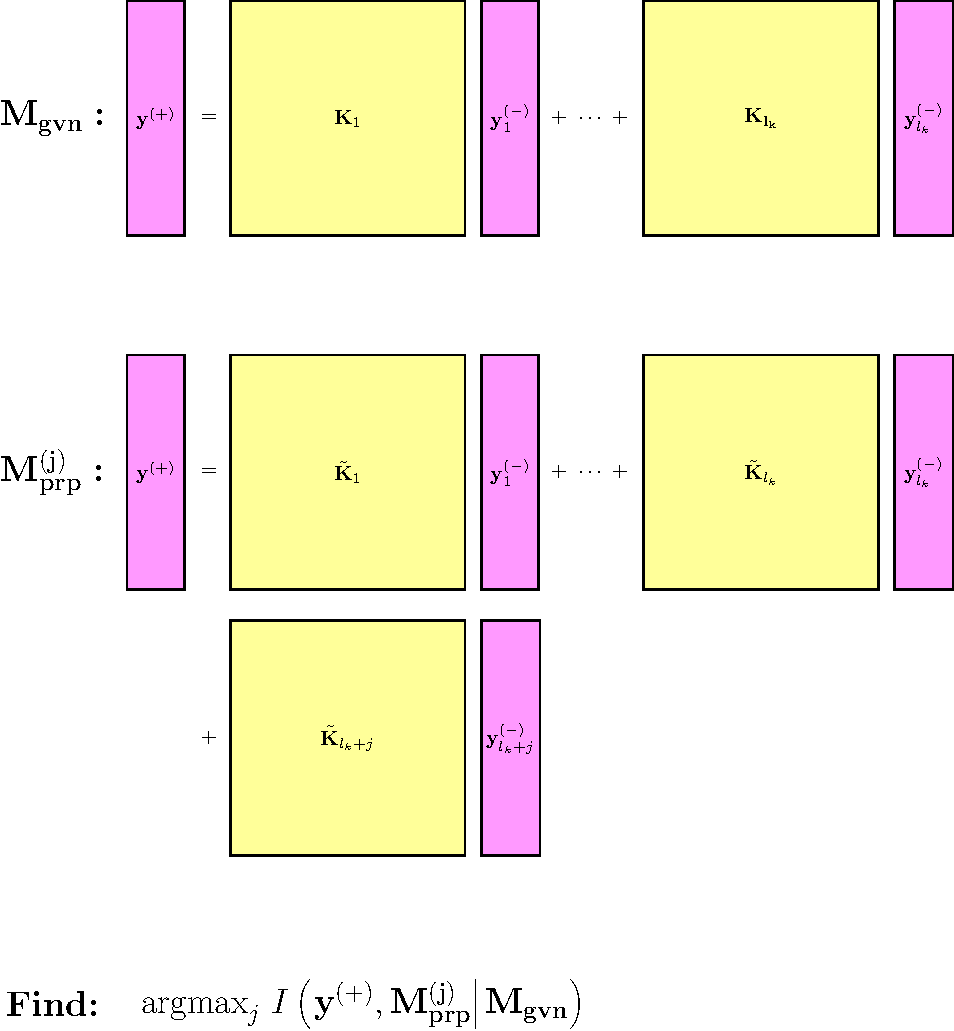
\includegraphics[scale=.75]{square_games-pics}
\end{figure}
Note, we always have $1\in l_{c}$ since this makes all subsequent lags improvements on the basic DMD approach.  This process is formalized and detailed in Algorithm \ref{erdmd}.  
\begin{algorithm}
\caption{ERDMD Method}
\begin{algorithmic}[1]
    \Procedure{Initialize}{}
        \State Set $l_{c}=\left\{1\right\}$ and $l_{r}=\left\{2, \cdots, d\right\}$.
        \State Find ${\bf K}_{1} =  \text{arg min}_{\bf K}\gnorm{{\bf Y}^{+}_{1}-{\bf K}{\bf Y}_{-}\left(l_{c}\right)}_{F}$.  Set ${\bf K}(l_{c})=({\bf K}_{1})$.
    \EndProcedure
\Procedure{Build}{}
		\While{$l_{r}\neq \left\{\varnothing\right\}$}
        \State Given $l_{c}=\left\{1~l_{1} \cdots l_{j}\right\}$, ${\bf K}({\bf l}_{c})$, and $l_{r}=\left\{2,\cdots,d\right\}\backslash l_{c}$        
        \For{$l_{j+1}\in l_{r}$}
        \State Define $l_{t}=l_{c}\cup \left\{l_{j+1}\right\}$ and find
        \[
        {\bf K}(l_{t}) = \text{arg min}_{\bf \tilde{K}_{1}, {\bf \tilde{K}}_{l_{1}}, \cdots {\bf \tilde{K}}_{l_{j+1}}}\gnorm{{\bf Y}^{+}_{l_{j+1}}-{\bf \tilde{K}}(l_{t}){\bf Y}_{-}(l_{t}) }_{F}.
        \]          
    \EndFor
    \State Choose $l_{j+1}$ and the corresponding $l_{t}$ and ${\bf K}(l_{t})$ to maximize
        \[
        I\left(\left. {\bf Y}^{+}_{d}, {\bf K}(l_{t}){\bf Y}_{-}(l_{t})\right|{\bf K}(l_{c}){\bf Y}_{-}(l_{t})\right)
        \]
        \State If choice is statistically significant, update $l_{c}$ and ${\bf K}(l_{c})$.
    \EndWhile
    \EndProcedure
    \Procedure{Prune}{}
        \State Given $l_{c}=\left\{1,l_{1}, \cdots, l_{N_{L}}\right\}$, set $S \equiv \text{True}$
        \While{$S$}
        \For{$l_{j}\in l_{c}$}
        	\State Define $l_{t}=\left\{1,l_{1}, \cdots, l_{N_{L}}\right\}\backslash \left\{l_{j}\right\}$
            \State Compute
            \[
            I\left(\left. {\bf Y}^{+}_{l_{N_{L}}}, {\bf K}(l_{t}){\bf Y}_{-}(l_{t})\right|{\bf K}(l_{c}){\bf Y}_{-}(l_{t})\right).
            \]
            
        \EndFor
        \State Choose $l_{t}$ corresponding to minimum information.  
        \If{minimum is statistically insignificant}
        \State Prune corresponding $l_{j}$ from $l_{c}$ and ${\bf K}(l_{c})$.
        \Else
        \State $S\equiv \text{False}$
        \EndIf
        \EndWhile
    \EndProcedure
\end{algorithmic}
\label{erdmd}
\end{algorithm}

\section{Results}
To study the efficacy of our method, we examine its use over numerically generated data from various chaotic dynamical systems.  In each case, for a given time series $\left\{{\bf y}_{j}\right\}_{j=0}^{N_{T}}$ we choose a maximum lag $d$ and then use a derived model to reconstruct the original time series after the $d^{th}$ step, i.e. $\left\{{\bf y}_{j}\right\}_{j=d}^{N_{T}}$. In each case, our models are from our proposed ERDMD method and the HODMD method.   

\subsection{Lorenz-63}
We now examine how well our method performs on the standard Lorenz-63 system, given by the equations
\begin{align*}
\dot{y}_{1} & = \sigma(y_{2}-y_{1})\\
\dot{y}_{2} & = y_{1}(\rho - y_{3}) - y_{2}\\
\dot{y}_{3} & = y_{1}y_{2}-\beta y_{3}\\
\end{align*}
with $\sigma=10$, $\rho=28$, and $\beta = 8/3$.  These parameter choices ensure that trajectories are pulled onto a strange attractor and exhibit chaotic dynamics.  We test our method on numerically generated data.  Time stepping is done with standard Runge--Kutta 4.For our numerics, the time step is $dt=.01$, and we run the simulation from $0\leq t \leq 22$.  

We look at data for $20\leq t \leq 22$, with $d=150$, corresponding to $1.5$ units of non-dimensional time.  We then compare our ER-DMD model to a model using all possible lags for $21.5\leq t \leq 22$.  The ERDMD algorithm converges to $l_{c}=\left\{1,149\right\}$.  The results are seen in Figure \ref{fig:lorenz_compare_d_150}.  As can be seen, all three curves are indistinguishable to the eye, showing that a far more minimal lag model is able to reconstruct dynamics with as much practical accuracy as the full HODMD method.  Further, looking beyond the reconstruction to the forecast regime, we see the ERDMD model does a generally better job beyond the data, thereby implying that the HODMD model is overfitting.  
\begin{figure}[!h]
\centering
\begin{tabular}{c}
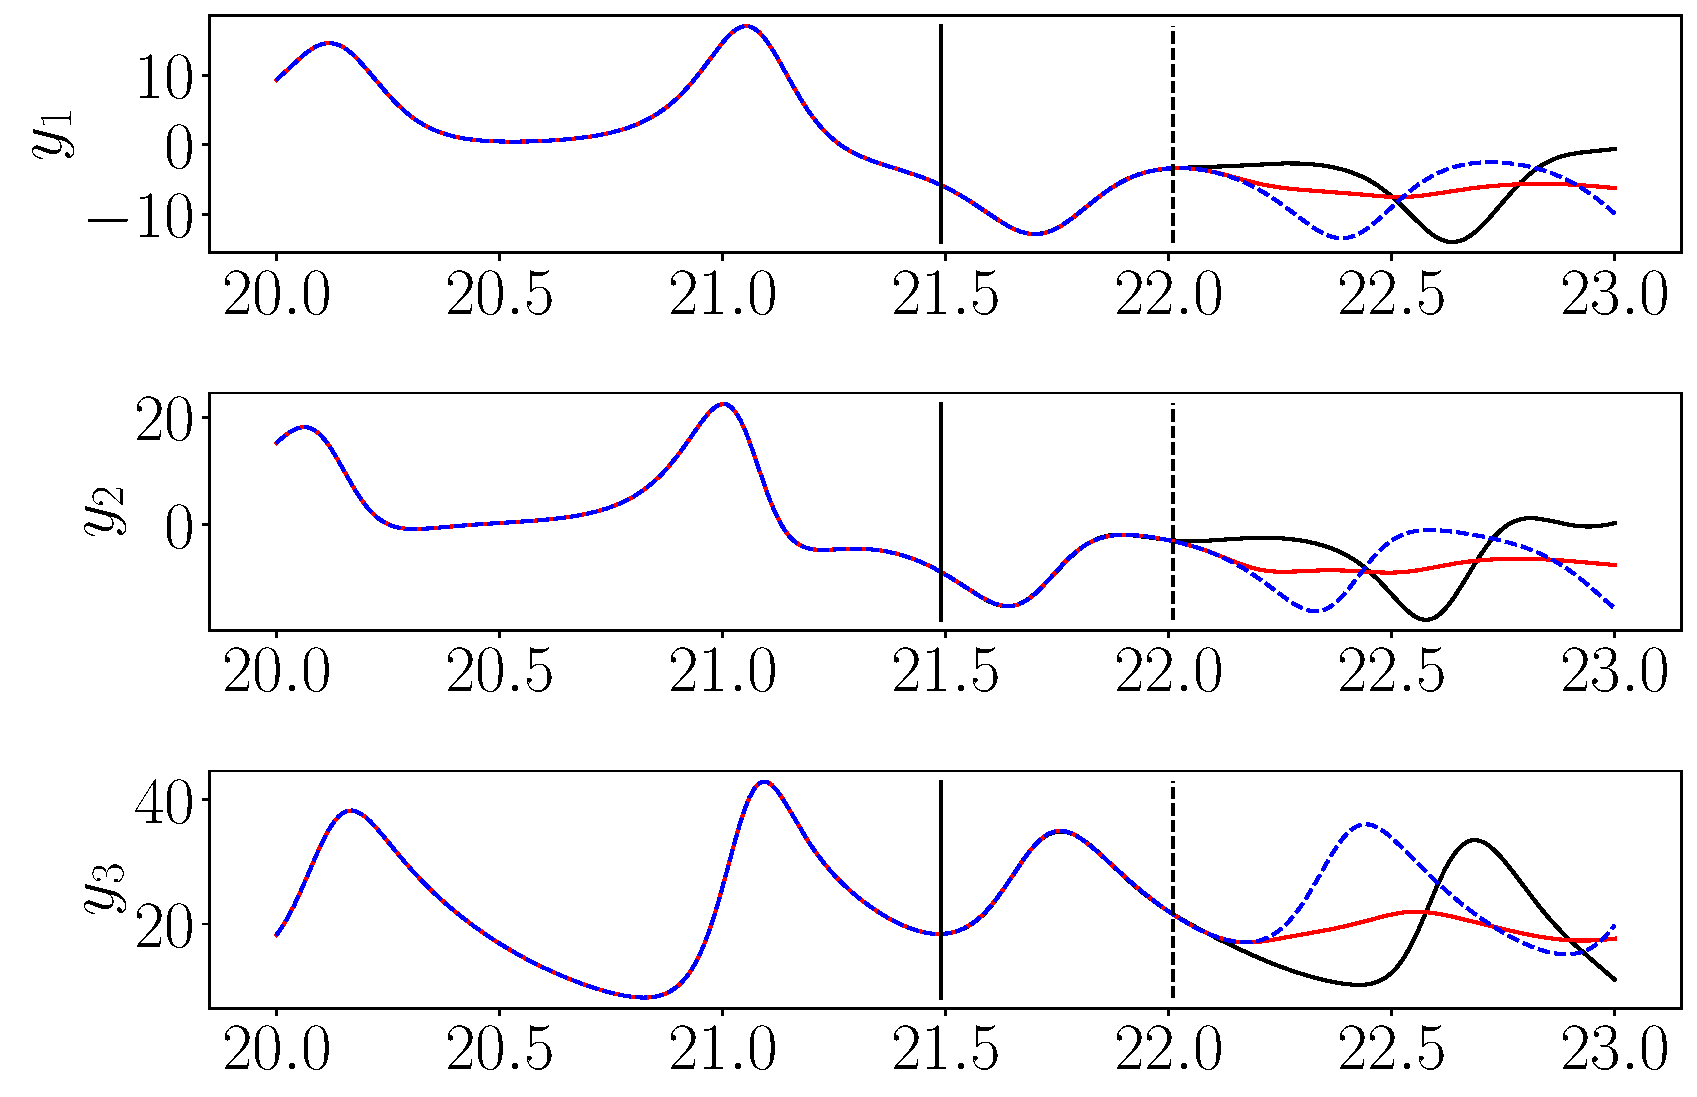
\includegraphics[width=.8\textwidth]{Lorenz_compare_w_mx_lag_150}\\
(a) Trajectories\\
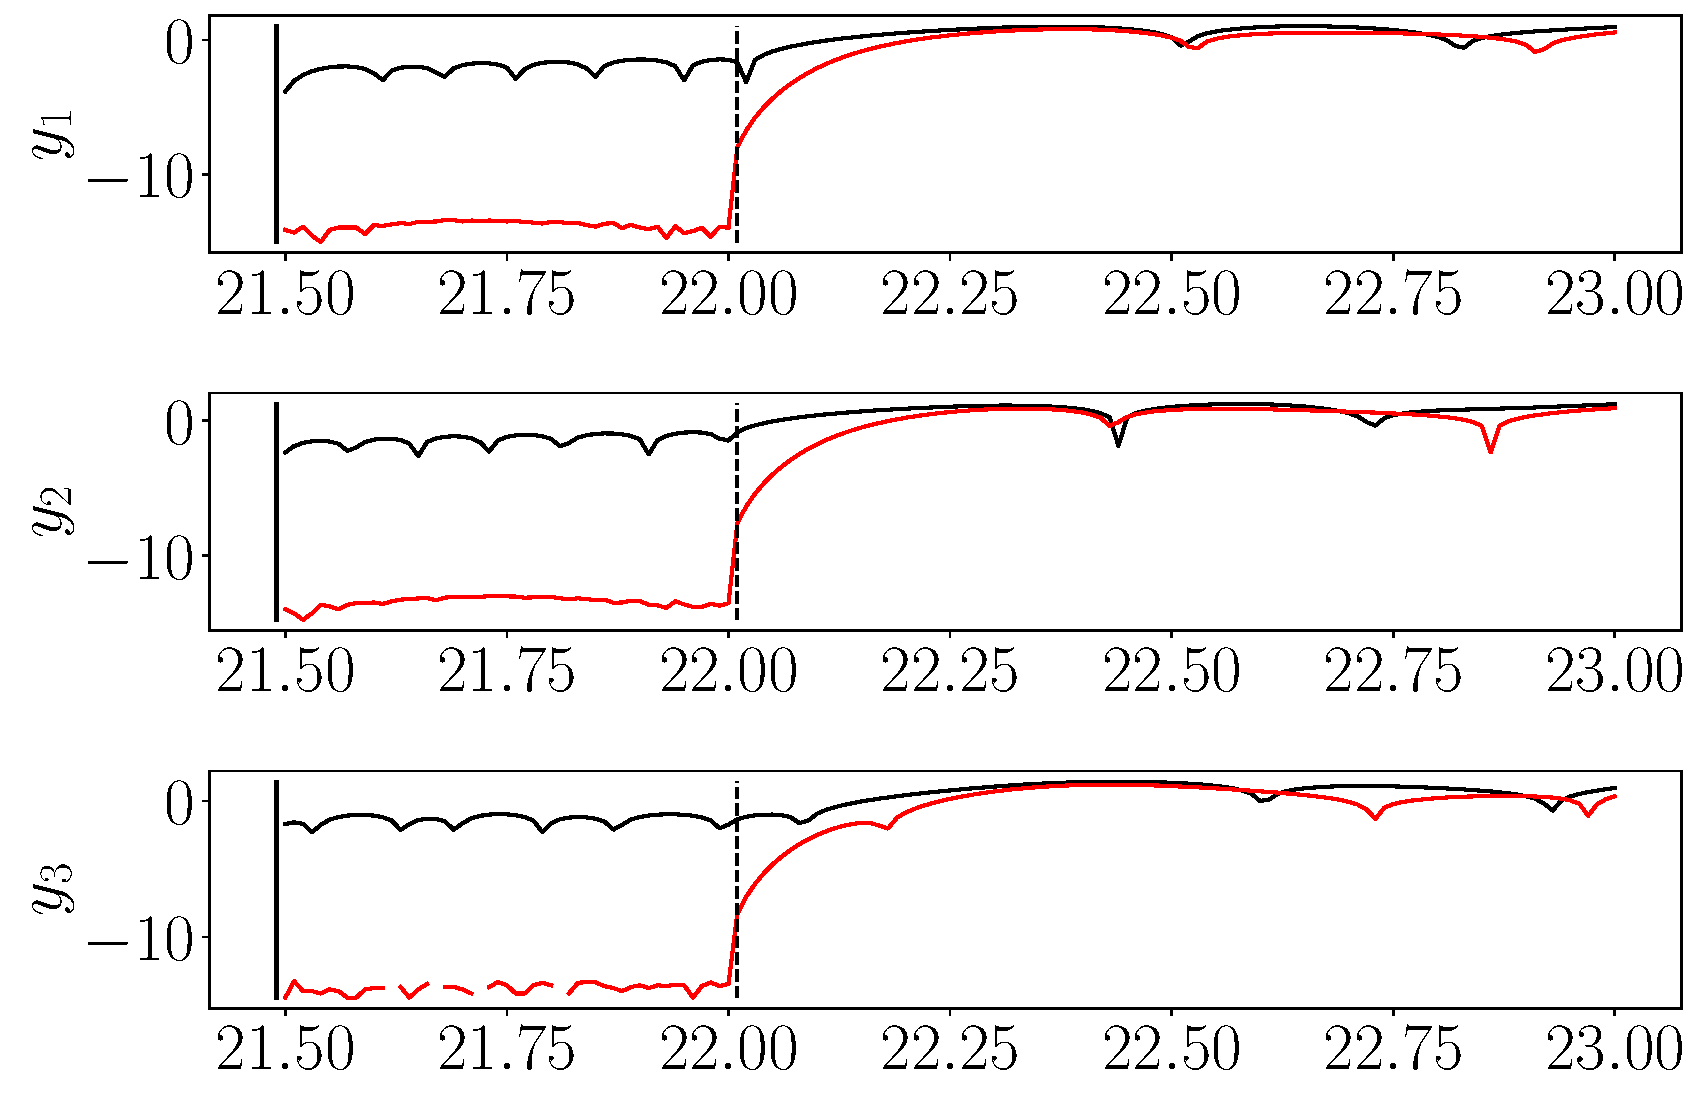
\includegraphics[width=.8\textwidth]{Lorenz_error_compare_w_mx_lag_150}\\
(b) Error Comparison (semi-log scale)
\end{tabular}
\caption{Direct comparison of ERDMD and all lags HODMD model against the true trajectory for the Lorenz-63 system (a), and error across dimensions for the ERDMD and all lags HODMD method (b).  The black line indicates the ERDMD result while the red indicates the all lags HODMD result.  The solid vertial bar indicates the maximum lag choice of $d=150$, while the dashed line indicates the end of the reconstruction interval and the beginning of the forecasting regime. The ERDMD algorithm converges to $l_{c}=\left\{1,149\right\}$.}
\label{fig:lorenz_compare_d_150}
\end{figure}

To this end, we can also compare the models generated by ERDMD and HODMD.  Looking at the norms of the various lag matrices in Figure \ref{fig:model_comp_d_150} we see that the ERDMD model produces a much sparser model with significantly larger overall matrix norms.  Likewise, the relative continuity of magnitudes of the lag matrices of the HODMD method allows for some description of the preferred scales of the model, but it is nowhere near as clear as when using ERDMD to accomplish the same task.  
\begin{figure}[!h]
\centering
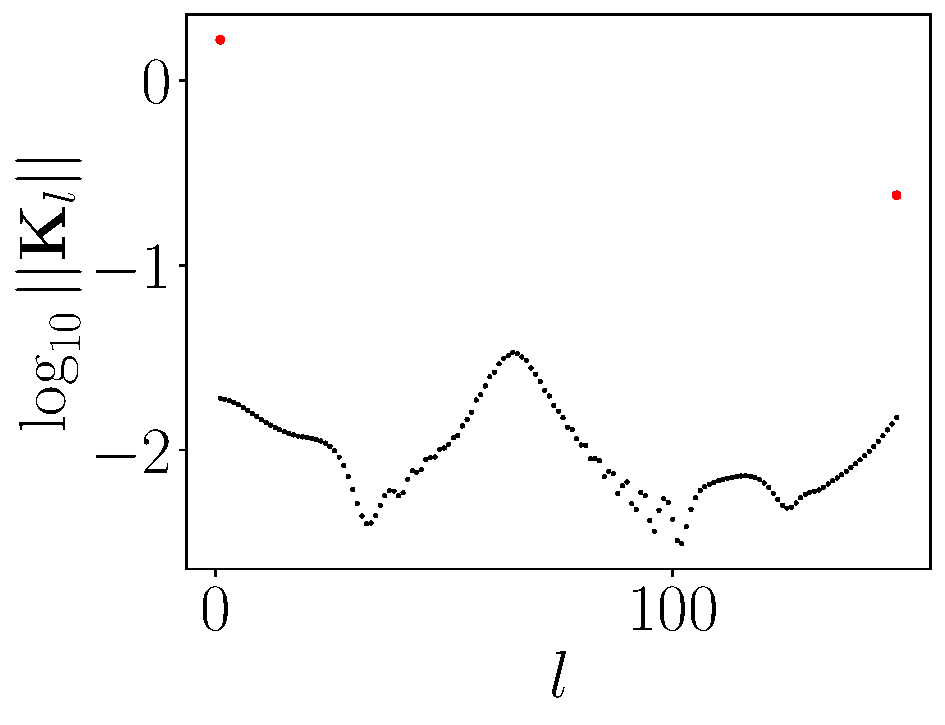
\includegraphics[width=.7\textwidth]{Lorenz_norm_full_model_149}
\caption{Comparison of the HODMD lagged matrix norms (black dots) and the ERDMD model (red dots).}
\label{fig:model_comp_d_150}
\end{figure}

Constructing the full Koopman one-step approximation ${\bf K}_{a}$ as in Equation \eqref{full_matrix} allows us to find the affiliated Koopman spectrum as seen in the left side of Figure \ref{fig:lorenz_spectrum_d_150}.  
\begin{figure}[!h]
\centering
\begin{tabular}{c}
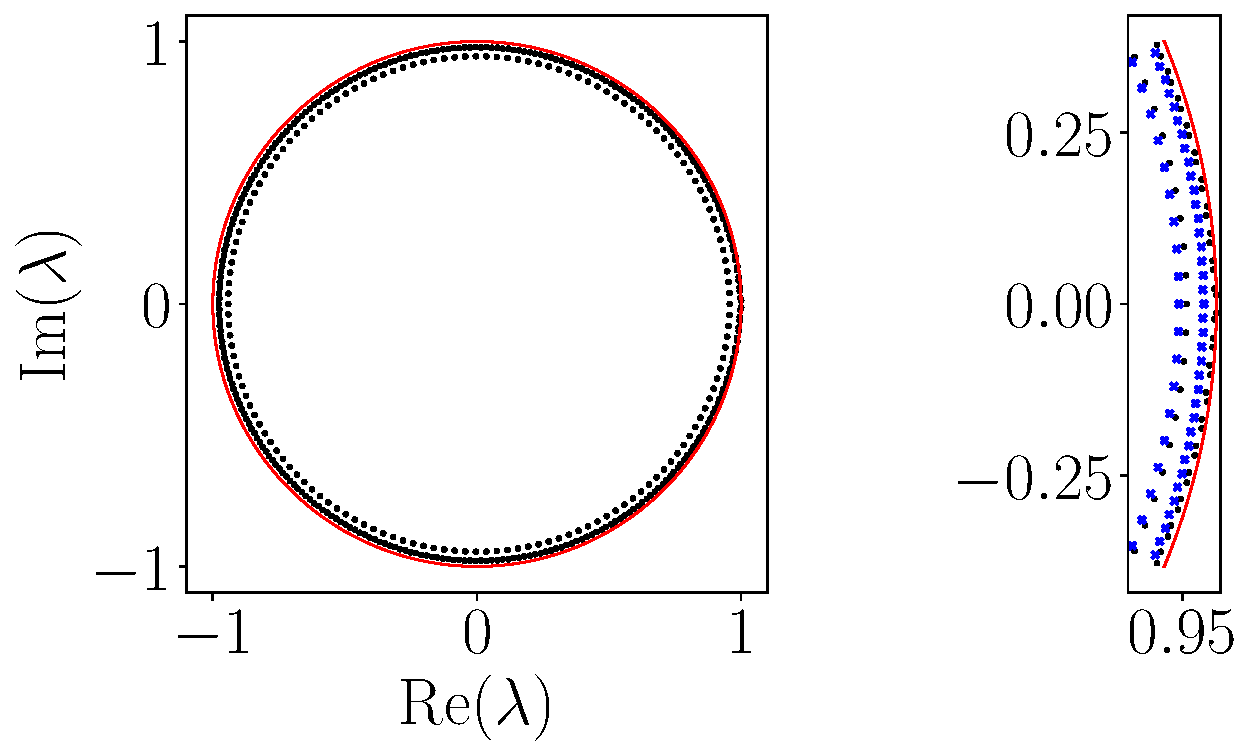
\includegraphics[width=1\textwidth]{Lorenz_detail_spectrum_w_mx_lag_149}
\end{tabular}
\caption{Spectrum of corresponding ERDMD Koopman operator for Lorenz-63 with $d=150$ on the left side, with a detail comparison to the reduced approximation (blue crosses) on the right side near (1,0).  The ERDMD algorithm converges to $l_{c}=\left\{1,149\right\}$.  The solid/red line is the unit circle, provided for reference.}
\label{fig:lorenz_spectrum_d_150}
\end{figure}

We see that because of the strong separation in lags as seen in $l_{c}$ that the affiliated characteristic polynomial $p_{a}(z)$ is given explicitly by
\[
p_{a}(z) = \text{det}\left({\bf K}_{149} + \left({\bf K}_{1}-z{\bf I}\right)z^{148} \right).
\]
If we look at the interior of the unit disc so that $|z|<1$, then our innermost eigenvalues to leading order are found from the roots of $\tilde{p}_{a}(z)$ where
\[
\tilde{p}_{a}(z) = \text{det}\left({\bf K}_{149} + {\bf K}_{1}z^{148}\right)
\]
or the leading roots are found by finding the generalized eigenvalues $\tilde{z}=z^{148}$ of the two matrix problem ${\bf K}_{149} + {\bf K}_{1}\tilde{z}$.  Looking at this spectrum in Figure \ref{fig:lorenz_spectrum_d_150} (b), we see that most of the features in the spectrum seen in the full spectrum on the left are present in the right.  Thus, the damping in the dynamics comes almost entirely from the disparity in lag values.  Looking at Figure \ref{fig:lorenz_spectrum_d_150} (c), which shows a detailed comparison of the two spectra for complex phase $\phi$ such that $|\phi|<\frac{\pi}{8}$, we see that the full spectrum gets closer to the unit circle and even has two modes which just cross the unit circle.  Otherwise, the reduced model well describes the damping modes, though we also see that the lag matrices ${\bf K}_{1}$ and ${\bf K}_{149}$ balance for more delicate dynamics along the unit circle.    

By way of contrast though, if we set the maximum lag $d=100$, and build reconstructions for $21\leq t \leq 22$, we find that the ERDMD results differ  markedly in terms of the determined lags though ultimately not in terms of accuracy; see Figure \ref{fig:lorenz_compare_d_100}.  In this case, the ERDMD algorithm converges onto the lag choices 
$$
l_{c}=\left\{1,15, 26, 35, 45, 48, 68, 73, 97,99\right\}.
$$  By choosing a lag horizon which does not fully capture the approximate period of oscillation in the dynamics, we need significantly more information to accurately reconstruct the data, though still nowhere as much as the full HODMD model.  
\begin{figure}[!h]
\centering
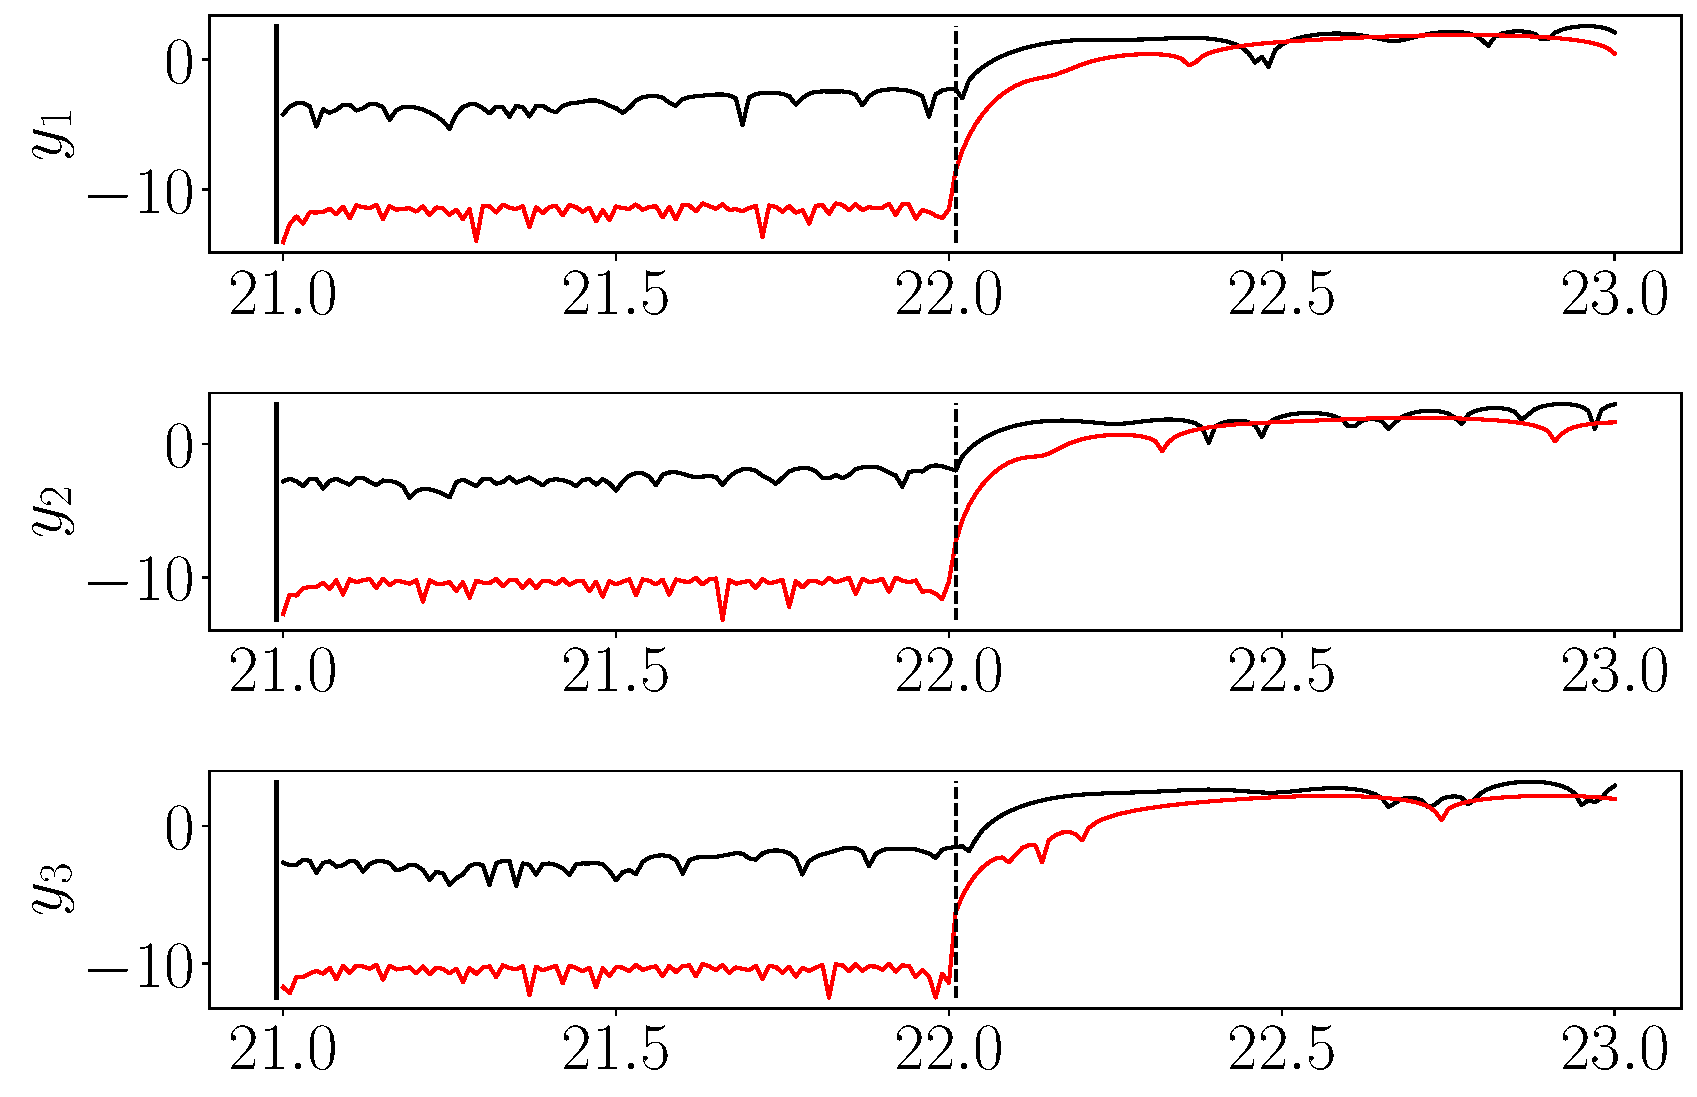
\includegraphics[width=.8\textwidth]{Lorenz_error_compare_w_mx_lag_100}
\caption{Comparison of ERDMD and all lags HODMD model against true trajectory for Lorenz-63 system.  The ERDMD reconstruction is in solid black in the figure.  The vertial bar indicates the maximum lag choice of $d=100$. The ERDMD algorithm converges to $l_{c}=\left\{1,15, 26, 35, 45, 48, 68, 73, 97,99\right\}$.}
\label{fig:lorenz_compare_d_100}
\end{figure}
 
Comparing the models again as seen in Figure \ref{fig:model_comp_d_99}, we see that for $d=100$ we get a less minimal ERDMD model though with markedly larger matrix norms for the longer lags, helping us to see that the model prioritizes long correlations in time in order to find accurate reconstructions.  Likewise, the full HODMD model has some degree of spread in magnitudes, but it does not allow for ready analysis or description.    
\begin{figure}[!h]
\centering
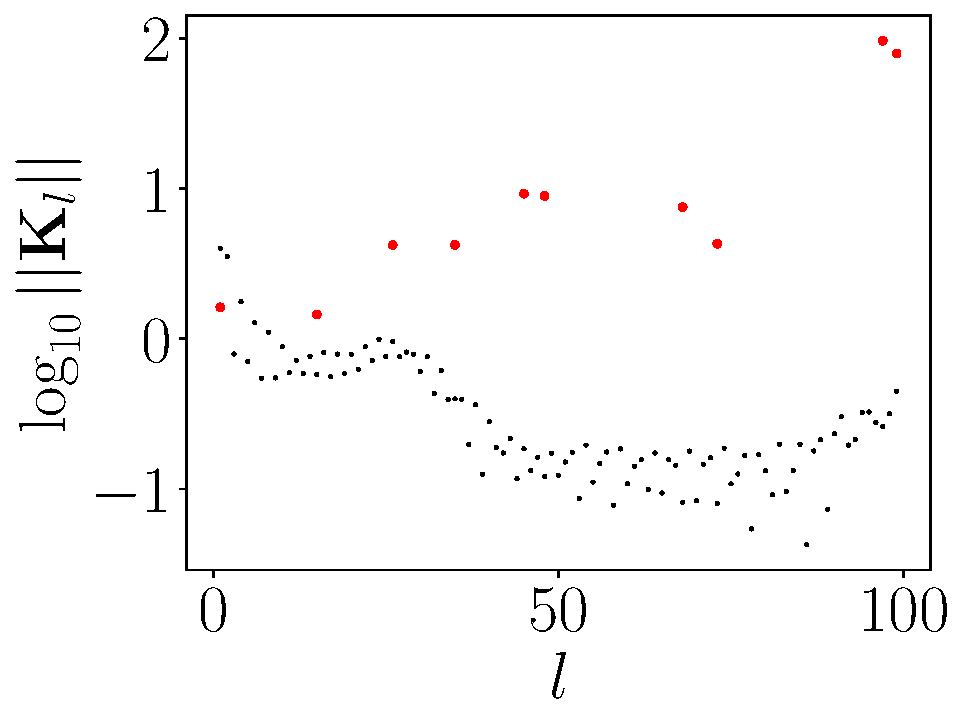
\includegraphics[width=.7\textwidth]{Lorenz_norm_full_model_99}
\caption{Comparison of the HODMD lagged matrix norms (black dots) and the ERDMD model (red dots).}
\label{fig:model_comp_d_99}
\end{figure}
 
We can likewise find the spectrum of ${\bf K}_{a}$ as seen in Figure \ref{fig:lorenz_spectrum_d_100}.  In this case, the larger spread of lags makes ready identification of positions in the spectrum to lag structure more difficult, though we see that 
\begin{figure}[!h]
\centering
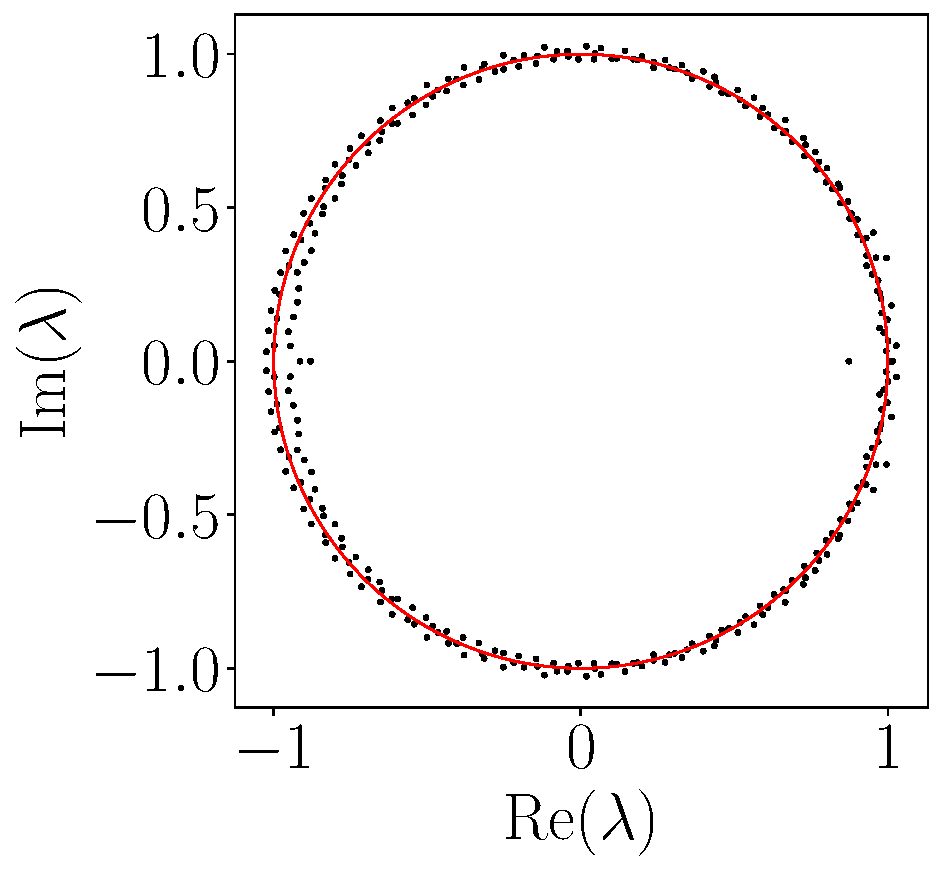
\includegraphics[width=.5\textwidth]{Lorenz_spectrum_w_mx_lag_99}
\caption{Spectrum of corresponding ERDMD Koopman operator for Lorenz-63 for $d=100$.  The ERDMD algorithm converges to $l_{c}=\left\{1,15, 26, 35, 45, 48, 68, 73, 97,99\right\}$.  The solid/red line is the unit circle, provided for comparison.}
\label{fig:lorenz_spectrum_d_100}
\end{figure}
The more uniform spread in lag values makes any estimates of the spectrum using reduced models less useful beyond identifying the most strongly damped modes.  


\subsection*{Rossler Equation}
To see how the ERDMD method works on problems with multiple scales, we now look at modeling dynamics coming from the Rossler system, given by the equations
\begin{align*}
\dot{y}_{1} & = -y_{2} - y_{3}\\
\dot{y}_{2} & = y_{1} + ay_{2}\\
\dot{y}_{3} & = b + y_{3}(y_{1}-c)\\
\end{align*} 
where $a=.1$, $b=.1$, $c=14$.  To see the role the multiple time scales play in this proble, letting $\epsilon=.1$, then we see $a=b=\epsilon$ and $c=1.4/\epsilon$.  Letting $\tau = t/\epsilon$ and setting $y_{3} = \epsilon^{2}\tilde{y}_{3}(t,\tau)$, to leading order, in $y_{1}$ and $y_{2}$ we find 
\[
\begin{pmatrix}y_{1} \\ y_{2}\end{pmatrix} = e^{\epsilon t/2}\begin{pmatrix}\cos(t) & -\sin(t) \\ \sin(t) & \cos(t)\end{pmatrix}\begin{pmatrix}y_{1,0} \\ y_{2,0}\end{pmatrix} + \mathcal{O}(\epsilon^{2}),
\]
so that we have $\mathcal{O}(1)$ planar oscillations complimented by slow growth away from the origin.  Likewise, in $\tilde{y}_{3}$ we find 
\[
\p_{\tau}\tilde{y}_{3} + \epsilon \p_{t}\tilde{y}_{3} = 1 - 1.4\tilde{y}_{3} + \epsilon y_{1}\tilde{y}_{3}.
\]
This then motivates the expansion 
\[
\tilde{y}_{3}(t,\tau) = c(t) e^{-1.4\tau} + \frac{1}{1.4}\left(1-e^{-1.4\tau} \right) + \epsilon \tilde{y}_{3,1}(t,\tau) + \cdots, 
\]
which, to remove secularities then gets us the equation for $c(t)$ of the form
\[
\frac{dc}{dt} = y_{1}(t)\left(c - \frac{1}{1.4} \right).
\]
So we have 
\[
c(t) = \frac{1}{1.4} + \left(c(0)-\frac{1}{1.4}\right)e^{\int_{0}^{t}y_{1}(s)ds},
\]
so that $\tilde{y}_{3}$ stays small until the slow growth in $y_{1}$ due to the $e^{\epsilon t/2}$ term pushes the dynamics out of the plane.  

We build reconstructions for $25\leq t \leq 40$.  To get accurate results, we chose $d=1000$, for which choice the method converged to the set $l_{c}$ with
\[
l_{c} = \left\{1, 3, 170, 436, 553, 665, 988\right\}.
\]
As can be seen in Figure \ref{fig:rossler}, our accuracy relies on capturing a full departure from the fast through the slow manifold.  This also explains the need for such a large choice of $d$ relative to what was used for the Lorenz-63 system.  
\begin{figure}[!h]
\centering
\begin{tabular}{c}
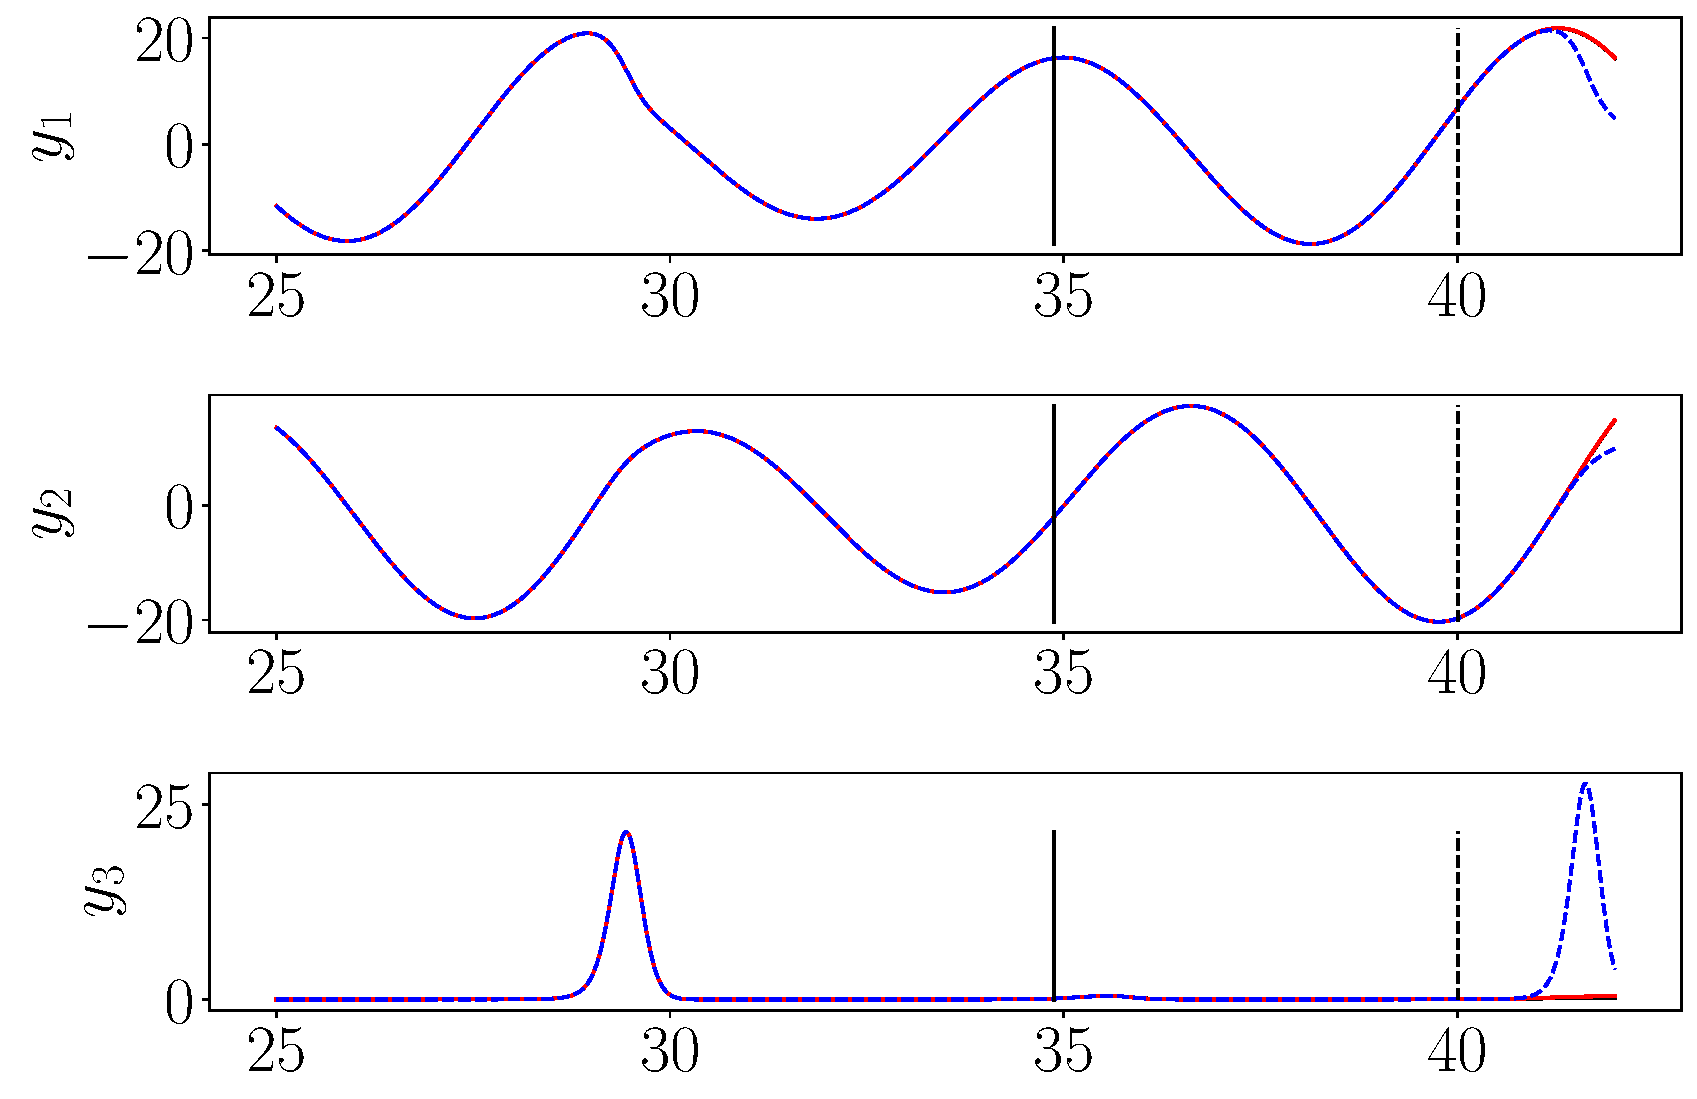
\includegraphics[width=.8\textwidth]{Rossler_compare_w_mx_lag_1000}\\
(a) Trajectories \\
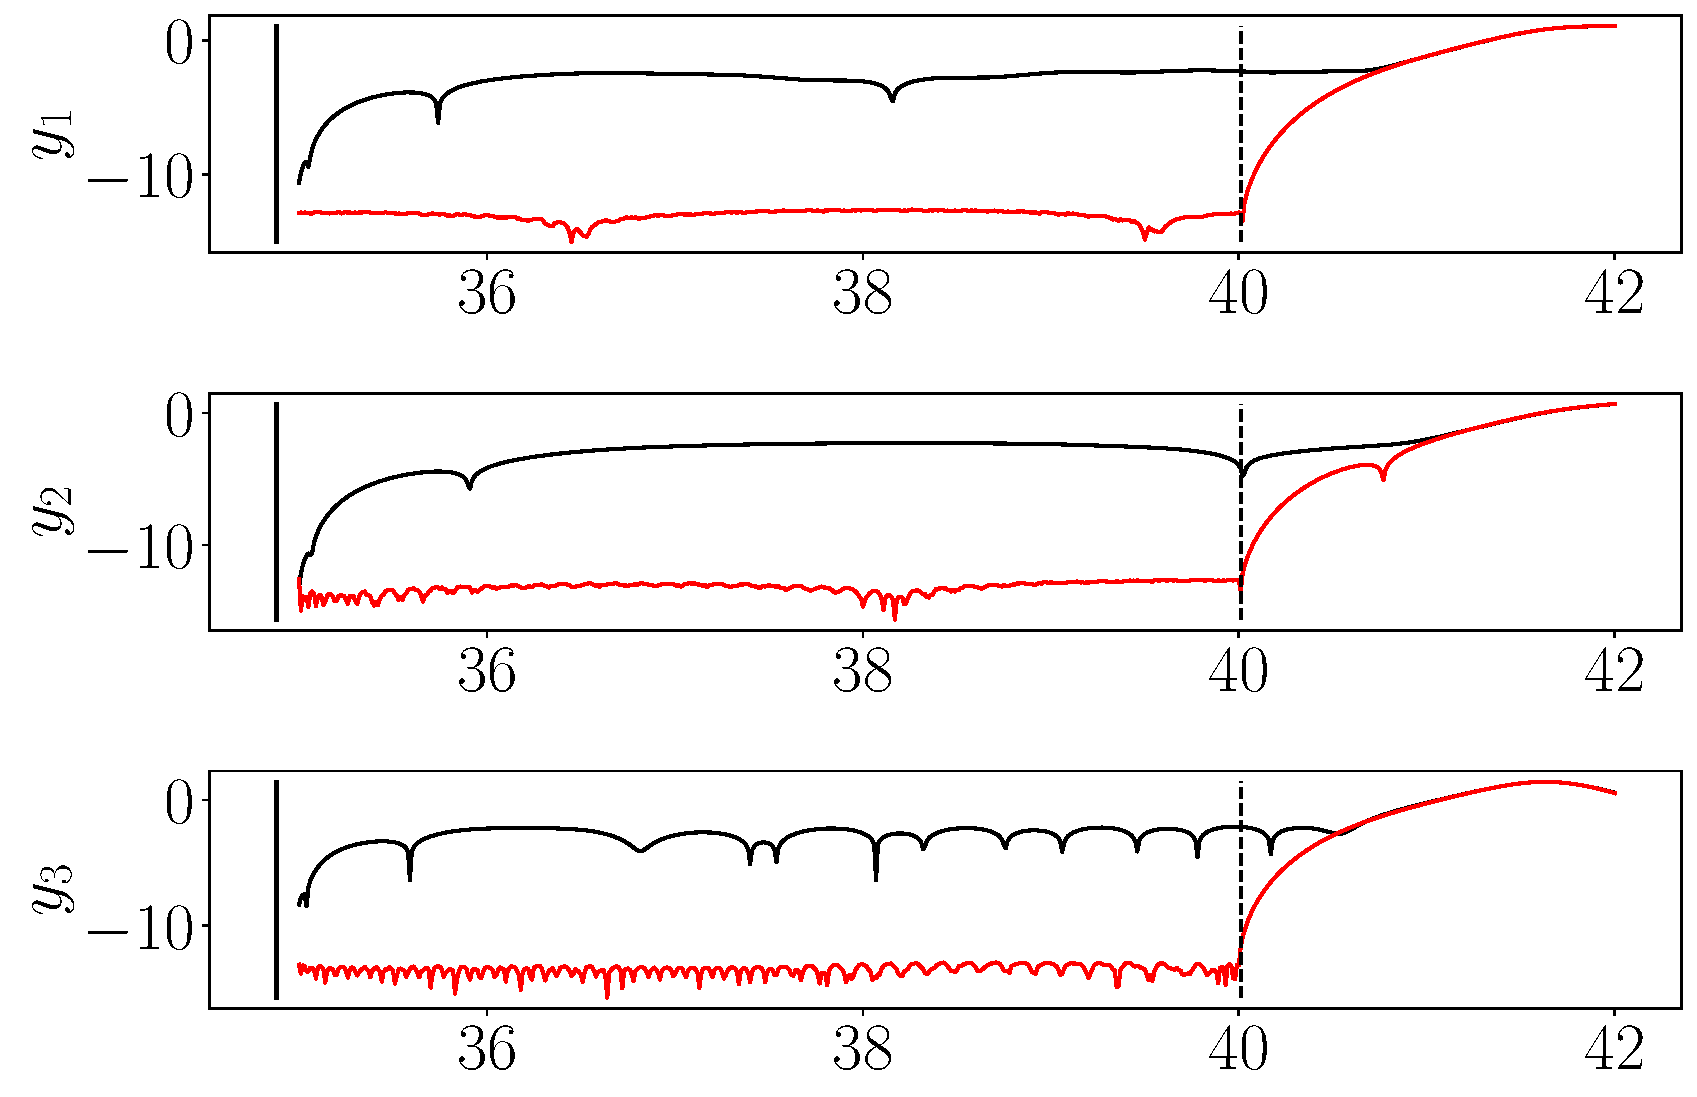
\includegraphics[width=.8\textwidth]{Rossler_error_compare_w_mx_lag_1000}\\
(b) Error Comparison
\end{tabular}
\caption{Comparison of ERDMD and all lags HODMD model against true trajectory for the Rossler system.  The ERDMD reconstruction is in solid black in the figure.  The vertial bar indicates the maximum lag choice of $d=1000$. The ERDMD algorithm converges to $l_{c}=\left\{1, 3, 170, 436, 553, 665, 988\right\}$.}
\label{fig:rossler}
\end{figure}

Comparing the HODMD and ERDMD models for the Rossler system, we see in Figure \ref{fig:model_comp_d_988} somewhat peculiar results.  Unlike for the Lorenz system, the norms of the lag matrices in the ERDMD model span ten order of magnitude.  Moreover, while ${\bf K}_{1}$ and ${\bf K}_{3}$ have relatively large norms, the remaining lag matrices are $10^{-10}$ times smaller, so all of the long time lag matrices are categorically miniscule in comparison.  So how can they have any meaningful impact within the model?  
\begin{figure}[!h]
\centering
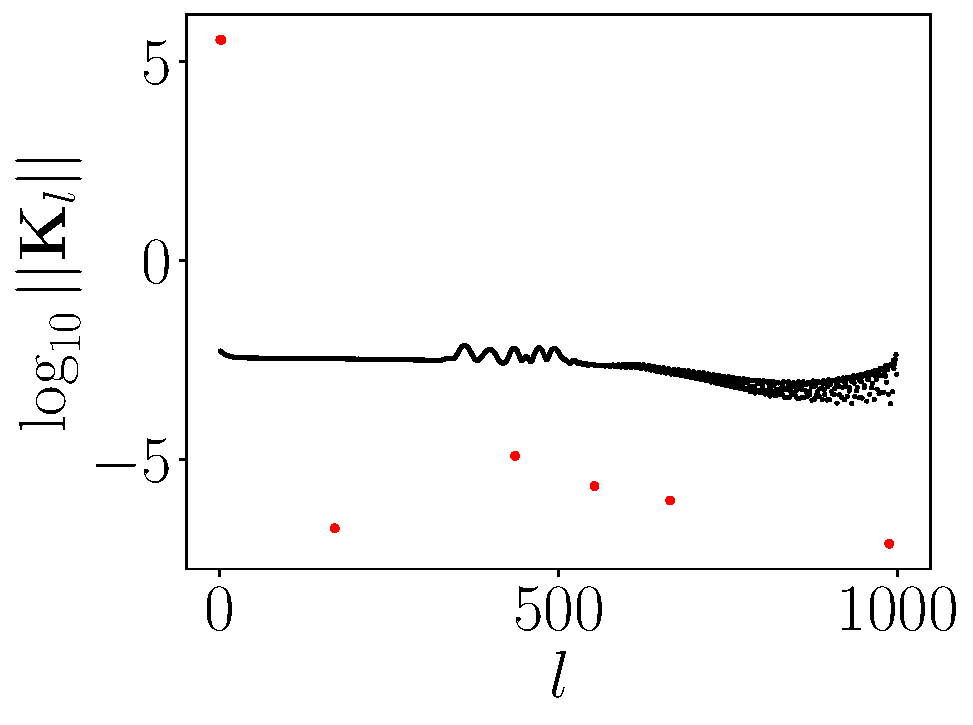
\includegraphics[width=.7\textwidth]{Rossler_norm_full_model_988}
\caption{Comparison of the HODMD lagged matrix norms (black dots) and the ERDMD model (red dots).}
\label{fig:model_comp_d_988}
\end{figure}

This question is answered in part by examining the spectrum, which will show us the spread in lag matrix norms is a result of the multiscale nature of the Rossler system.  This of course appears in the wide spread of values of the optimal lags we see in $l_{c}$.  So while we can find the affiliated spectrum as seen in Figure \ref{fig:rossler_spectrum}, we can also explore its structure in terms of the strongly separated lag values we find in $l_{c}$.  Looking for eigenvalues within the unit circle can be done by computing
\[
\tilde{p}_{a}(z) = \text{det}\left(z^{323}{\bf K}_{665} + {\bf K}_{988} \right)
\]
which corresponds to the slowest scales in our ERDMD model.  Likewise, if we look for eigenvalues outside the unit circle, we look to the fastest scales corresponding to the reduced polynomial
\[
\tilde{p}_{a}(z) = \text{det}\left(z^{3} - {\bf K}_{1}z^{2} - {\bf K}_{3}) \right)
\]

\begin{figure}[!h]
\centering
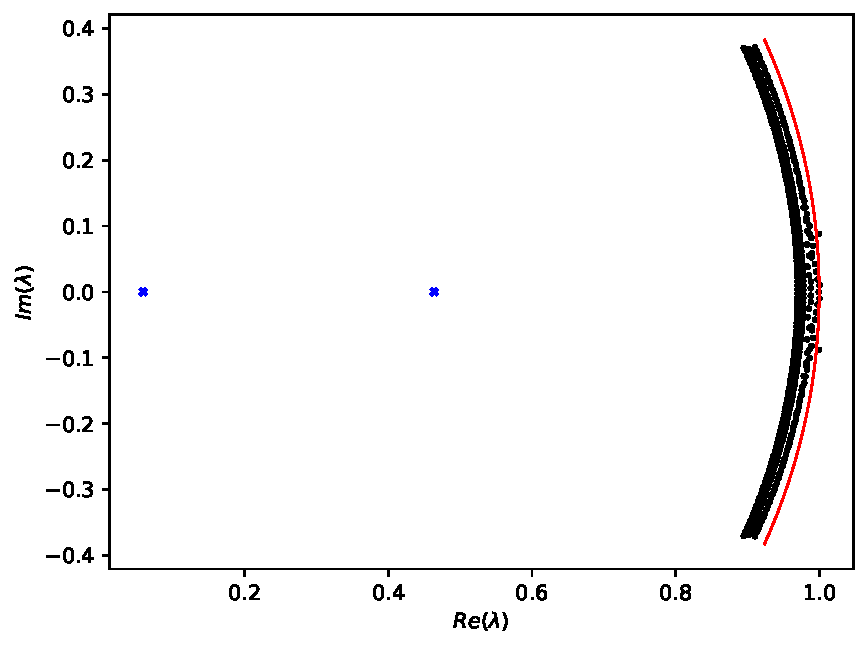
\includegraphics[width=1.\textwidth]{Rossler_detail_spectrum_w_mx_lag_988}\\
\caption{Spectrum of corresponding ERDMD Koopman operator for the Rossler system.  The ERDMD algorithm converges to $l_{c}= \left\{1, 3, 170, 436, 553, 665, 988\right\}$.  The solid/red line is the unit circle, provided for comparison.}
\label{fig:rossler_spectrum}
\end{figure}

\subsection*{Kuramoto--Sivashinsky Equation}
To look at a more intricate and higher dimensional example, we now study the Kuramoto--Sivashinsky (KS) equation given by 
\[
u_{t} + u_{xx} + u_{xxxx} + uu_{x} = 0, ~ u(x+2L,t) = u(x,t).
\]
See \cite{robinson} for an extensive bibliography with regards to details and relavent proofs of facts used in this paper.  Introducing the rescalings
\[
\tilde{t} =\frac{t}{T}, ~ \tilde{x} = \frac{\pi}{L}x, ~ u = A\tilde{u},
\]
and taking the balances
\[
A = \frac{L}{\pi T}, ~ T = \left(\frac{L}{\pi}\right)^{2}, 
\]
we get the equivalent KS equation (dropping tildes for ease of reading)
\[
u_{t} + u_{xx} + \nu u_{xxxx} + uu_{x} = 0, ~ \nu = \left(\frac{\pi}{L}\right)^{2}.
\]
Looking at the linearized dispersion relationship $\omega(k) = k^{2} - \nu k^{4}$, we see that the $\nu$ parameter acts as a viscous damping term.  Thus, as the system size $L$ is increased, the effective viscosity is decreased, thereby allowing for more complex dynamics to emerge.  As is now well known, for $L$ sufficiently large, a fractional-dimensional-strange attractor forms which both produces intricate spatio-temporal dynamics while also allowing for a far simpler representation of said dynamics.  It is has been shown in many different works (see for example \cite{citanovic}) that $L=11$ generates a strange attractor with dimension between eight and nine, and that this is about the smallest value of $L$ which is guaranteed to generate chaotic dynamics.  We therefore set $L=11$ throughout the remainder of this section.  

To study ERDMD on the KS equation, we use KS data numerically generated by a pseudo-spectral in space and fourth-order exponential-differencing Runge-Kutta in time method \cite{kassam} of lines approach.  For the pseudo-spectral method, $K=128$ total modes are used giving an effective spatial mesh width of $2L/K = .172$, while the time step for the Runge-Kutta scheme is set to $\delta t = .25$.  After a burn in time of $t_{b}=10$, we generated a simulation of length $t_{f} = \left(L/\pi\right)^{4}\approx 160$ to allow for nonlinear effects to fully manifest.  This trajectory was then separated via a POD into space and time modes; see \cite{berkooz}.  Taking $N_{s}=12$ modes captured 98.6\% of the total energy.  

To study the ERDMD method, we choose $d=200$, which for $dt=.25$ corresponds to a lag time of $t=60$.  With this choice, the ERDMD method finds $l_{c}$ to be 
\[
l_{c}=\left\{1, 123, 141, 158\right\}.
\]
The results for reconstruction can be seen in Figure \ref{fig:ks_compare_d_200}, we where we look at times $10\leq t \leq 66$.  As can be seen, the ERDMD does quite well, though we note that if we look for longer reconstructions, errors do start to appear more rapidly for the ERDMD method than the full HODMD method.  
\begin{figure}[!h]
\centering
\includegraphics[width=1\textwidth]{ks_dynamics_compare}
\caption{Comparison of ERDMD and all lags HODMD model against true trajectory for the KS equation.  The vertial bar indicates the maximum lag choice of $d=200$. The ERDMD algorithm converges to $l_{c}=\left\{1, 123, 141, 158\right\}$.}
\label{fig:ks_compare_d_200}
\end{figure} 
 
We see in Figure \ref{fig:ksspectrum} (a) the corresponding full spectrum affiliated with our method.  Again, the strong separation of lags in $l_{c}$ motivate looking at the roots of the reduced polynomial
\[
\tilde{p}_{a}(z) = \text{det}\left(z^{35}{\bf K}_{123} + z^{17}{\bf K}_{141} + {\bf K}_{158} \right).
\] 
Note, letting $\tilde{z}=z^{17}$, we can write 
\[
z^{35} = \tilde{z}^{2}e^{\ln \tilde{z}/17} \approx \tilde{z}^{2}
\]
so long as $|z|$ is not too close to zero.  We can then find the affiliated approxmiate companion matrix representation for $\tilde{p}_{a}(z)$ in the form
\[
\tilde{{\bf K}}_{a} = 
\begin{pmatrix} 
0 & I \\ 
-\tilde{{\bf K}}_{2} & -\tilde{{\bf K}}_{1} \\
\end{pmatrix}
\]
where 
\[
\tilde{{\bf K}}_{1} = {\bf K}_{123}^{-1}{\bf K}_{141}, ~ \tilde{{\bf K}}_{2} = {\bf K}_{123}^{-1}{\bf K}_{158}.
\]
The reduced spectrum is seen in Figure \ref{fig:ksspectrum} (b), where we again can see the most damped modes come from the highest lags in our Koopman model.  We can also look at the case of $|z|>1$, in which case our asymptotic arguments would lead us to just look at the largest eigenvalues of ${\bf K}_{1}$.  These results are compared in Figure \ref{fig:ksspectrum} (c), where we see the most unstable modes of the full spectrum correspond to the largest magnitude eigenvalues of ${\bf K}_{1}$.  Thus there is a clear separation in the Koopman spectrum across lag values, which is to say time scales in the dynamics.     
\begin{figure}[!h]
\centering
\begin{tabular}{c}
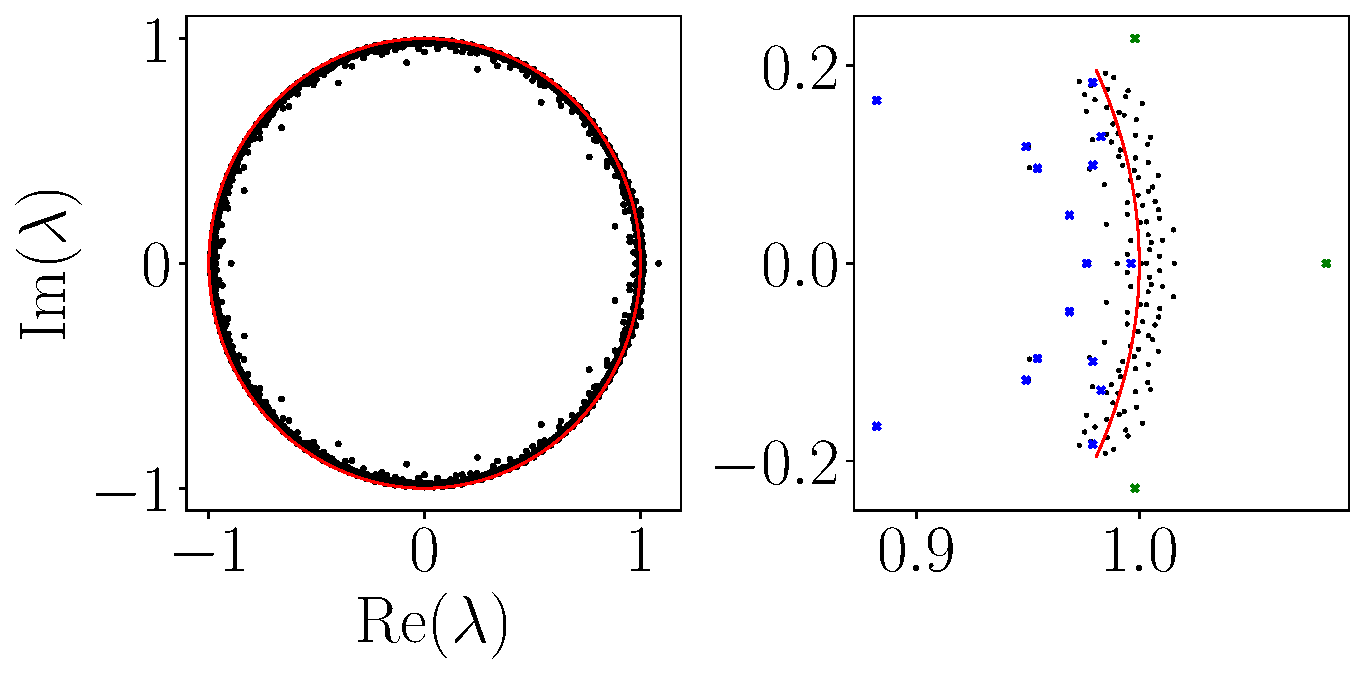
\includegraphics[width=1\textwidth]{Kuramoto_detail_spectrum_w_mx_lag_158} \end{tabular}
\caption{Full spectrum (left side) and detail comparson to the reduced spectrum (right side) of the corresponding ERDMD Koopman operator for Kuramoto--Sivashinsky.  The ERDMD algorithm converges to $l_{c}=\left\{1, 123, 141, 158\right\}$.  The solid/red line is the unit circle, which is provided for reference. In the detail comparison, we compare the full spectrum (black/dots) to the interior reduced approximation (blue/x) and the outer reduced approximation (green/x) in a region with angular apperature of $\pi/4$.}
\label{fig:ksspectrum}
\end{figure}

\section{Discussion}
Discuss discuss discuss.
\section*{Acknowledgements}
\bibliographystyle{unsrt}
\bibliography{ionosphere_bib}
\end{document}
